%% LyX 2.2.2 created this file.  For more info, see http://www.lyx.org/.
%% Do not edit unless you really know what you are doing.
\documentclass[twocolumn,english,prl, amsmath,amssymb,aps,superscriptaddress]{revtex4-1}
\usepackage[latin9]{inputenc}
\setcounter{secnumdepth}{3}
\usepackage{amsmath}
\usepackage{graphicx}

\makeatletter
%%%%%%%%%%%%%%%%%%%%%%%%%%%%%% User specified LaTeX commands.
% ****** Start of file apssamp.tex ******
%
%   This file is part of the APS files in the REVTeX 4.1 distribution.
%   Version 4.1r of REVTeX, August 2010
%
%   Copyright (c) 2009, 2010 The American Physical Society.
%
%   See the REVTeX 4 README file for restrictions and more information.
%
% TeX'ing this file requires that you have AMS-LaTeX 2.0 installed
% as well as the rest of the prerequisites for REVTeX 4.1
%
% See the REVTeX 4 README file
% It also requires running BibTeX. The commands are as follows:
%
%  1)  latex apssamp.tex
%  2)  bibtex apssamp
%  3)  latex apssamp.tex
%  4)  latex apssamp.tex
%


% Include figure files
\usepackage{dcolumn}% Align table columns on decimal point
\usepackage{bm}% bold math
%\usepackage{hyperref}% add hypertext capabilities
%\usepackage[mathlines]{lineno}% Enable numbering of text and display math
%\linenumbers\relax % Commence numbering lines

%\usepackage[showframe,%Uncomment any one of the following lines to test 
%%scale=0.7, marginratio={1:1, 2:3}, ignoreall,% default settings
%%text={7in,10in},centering,
%%margin=1.5in,
%%total={6.5in,8.75in}, top=1.2in, left=0.9in, includefoot,
%%height=10in,a5paper,hmargin={3cm,0.8in},
%]{geometry}

\makeatother

\usepackage{babel}
\begin{document}

\title{Direct verification of the fluctuation-dissipation relation in viscously
coupled oscillators}

\author{Shuvojit Paul$ $}

\affiliation{Indian Institute of Science Education and Research, Kolkata}

\author{Abhrajit Laskar}

\affiliation{The Institute of Mathematical Sciences-HBNI, CIT Campus, Taramani,
Chennai 600113, India}

\author{Rajesh Singh}

\affiliation{The Institute of Mathematical Sciences-HBNI, CIT Campus, Taramani,
Chennai 600113, India}

\author{Basudev Roy}

\affiliation{Department of Physics, Indian Institute of Technology Madras, Chennai
600036, India}

\author{R. Adhikari}
\email{rjoy@imsc.res.in}


\affiliation{The Institute of Mathematical Sciences-HBNI, CIT Campus, Taramani,
Chennai 600113, India}

\affiliation{DAMTP, Centre for Mathematical Sciences, University of Cambridge,
Wilberforce Road, Cambridge CB3 0WA, UK}

\author{Ayan Banerjee}
\email{ayan@iiserkol.ac.in}


\affiliation{Indian Institute of Science Education and Research, Kolkata}

\date{\today}
\begin{abstract}
The fluctuation-dissipation relation, a central result in non-equilibrium
statistical physics, relates equilibrium fluctuations in a system
to its linear response to external forces. Here we provide a direct
experimental verification of this relation for viscously coupled oscillators,
as realized by a pair of optically trapped colloidal particles. A
theoretical analysis, in which interactions mediated by slow viscous
flow are represented by non-local friction tensors, matches experimental
results and reveals a frequency maximum in the amplitude of the mutual
response which is a sensitive function of the trap stiffnesses and
the friction tensors. This allows for its location and width to be
tuned and suggests the utility of the trap setup for accurate two-point
microrheology.
\end{abstract}

\pacs{Valid PACS appear here}

\maketitle
The relation between the generalized susceptibility and equilibrium
fluctuations of the generalized forces, first obtained for a linear
resistive circuit by Nyquist \cite{nyquist1928thermal} and then proved
for any general linear dissipative system by Callen and Welton \cite{callen1951},
is a central result in non-equilibrium statistical physics. The relation
can be used to infer the intrinsic fluctuations of a system from measurements
of its response to external perturbations or, perhaps more startlingly,
to predict its response to external perturbations from the character
of its intrinsic fluctuations \cite{kubo1966fluctuation}. The fluctuation-dissipation
relation is the point of departure for several areas of current research
including fluctuation relations, relaxation in glasses, and response
and correlations in active and driven systems \cite{mason95,levine2000}. 

The first experimental\emph{ }verification of the relation between
fluctuation and dissipation was due to Johnson \cite{johnson1928thermal},
whose investigation of the ``thermal agitation of electricity in
conductors'' provided the motivation for Nyquist's theoretical work
\cite{nyquist1928thermal}. Though the relation has been verified
since in systems with conservative couplings, a direct verification
in a system where the coupling is entirely dissipative is, to the
best of our knowledge, not available. Colloidal particles in a viscous
fluid interact through velocity-dependent many-body hydrodynamic forces
whose strength, away from boundaries, is inversely proportional to
the distance between the particles. The range of these dissipative
forces can be made much greater than that of conservative forces such
as the DLVO interaction \cite{derjaguin1941theory,verwey1948}. Therefore,
it is possible to engineer a situation where the dominant coupling
between colloidal particles is the viscous hydrodynamic force and
all other interactions are negligibly small. Such systems, then, are
ideal for testing the fluctuation-dissipation relation when couplings
are purely dissipative. 

In this Letter, we present a direct verification of the fluctuation-dissipation
relation for a pair of optically trapped colloidal particles in water.
We measure the equilibrium fluctuations of the distance between the
particles and the response of one particle to the sinusoidal motion
of another particle. Transforming both correlations and responses
to the frequency domain, we verify the fluctuation-dissipation relation
over a range of frequencies spanning two orders of magnitude. Remarkably,
the response function has a peak in frequency, reminiscent of a resonance,
though the system of oscillators is entirely overdamped. A theoretical
analysis, assuming slow viscous flow of the ambient water, is in excellent
agreement with the experiments. The analysis reveals that the location
and width of the resonant peak can be tuned by altering the viscosity,
the separation between the particles, the trap stiffnesses, and the
colloidal diameters. It provides the inverse relations necessary for
using the trap setup for accurate two-point microrheology. We now
present details of our experiment and its analysis.

\begin{figure}
\centering 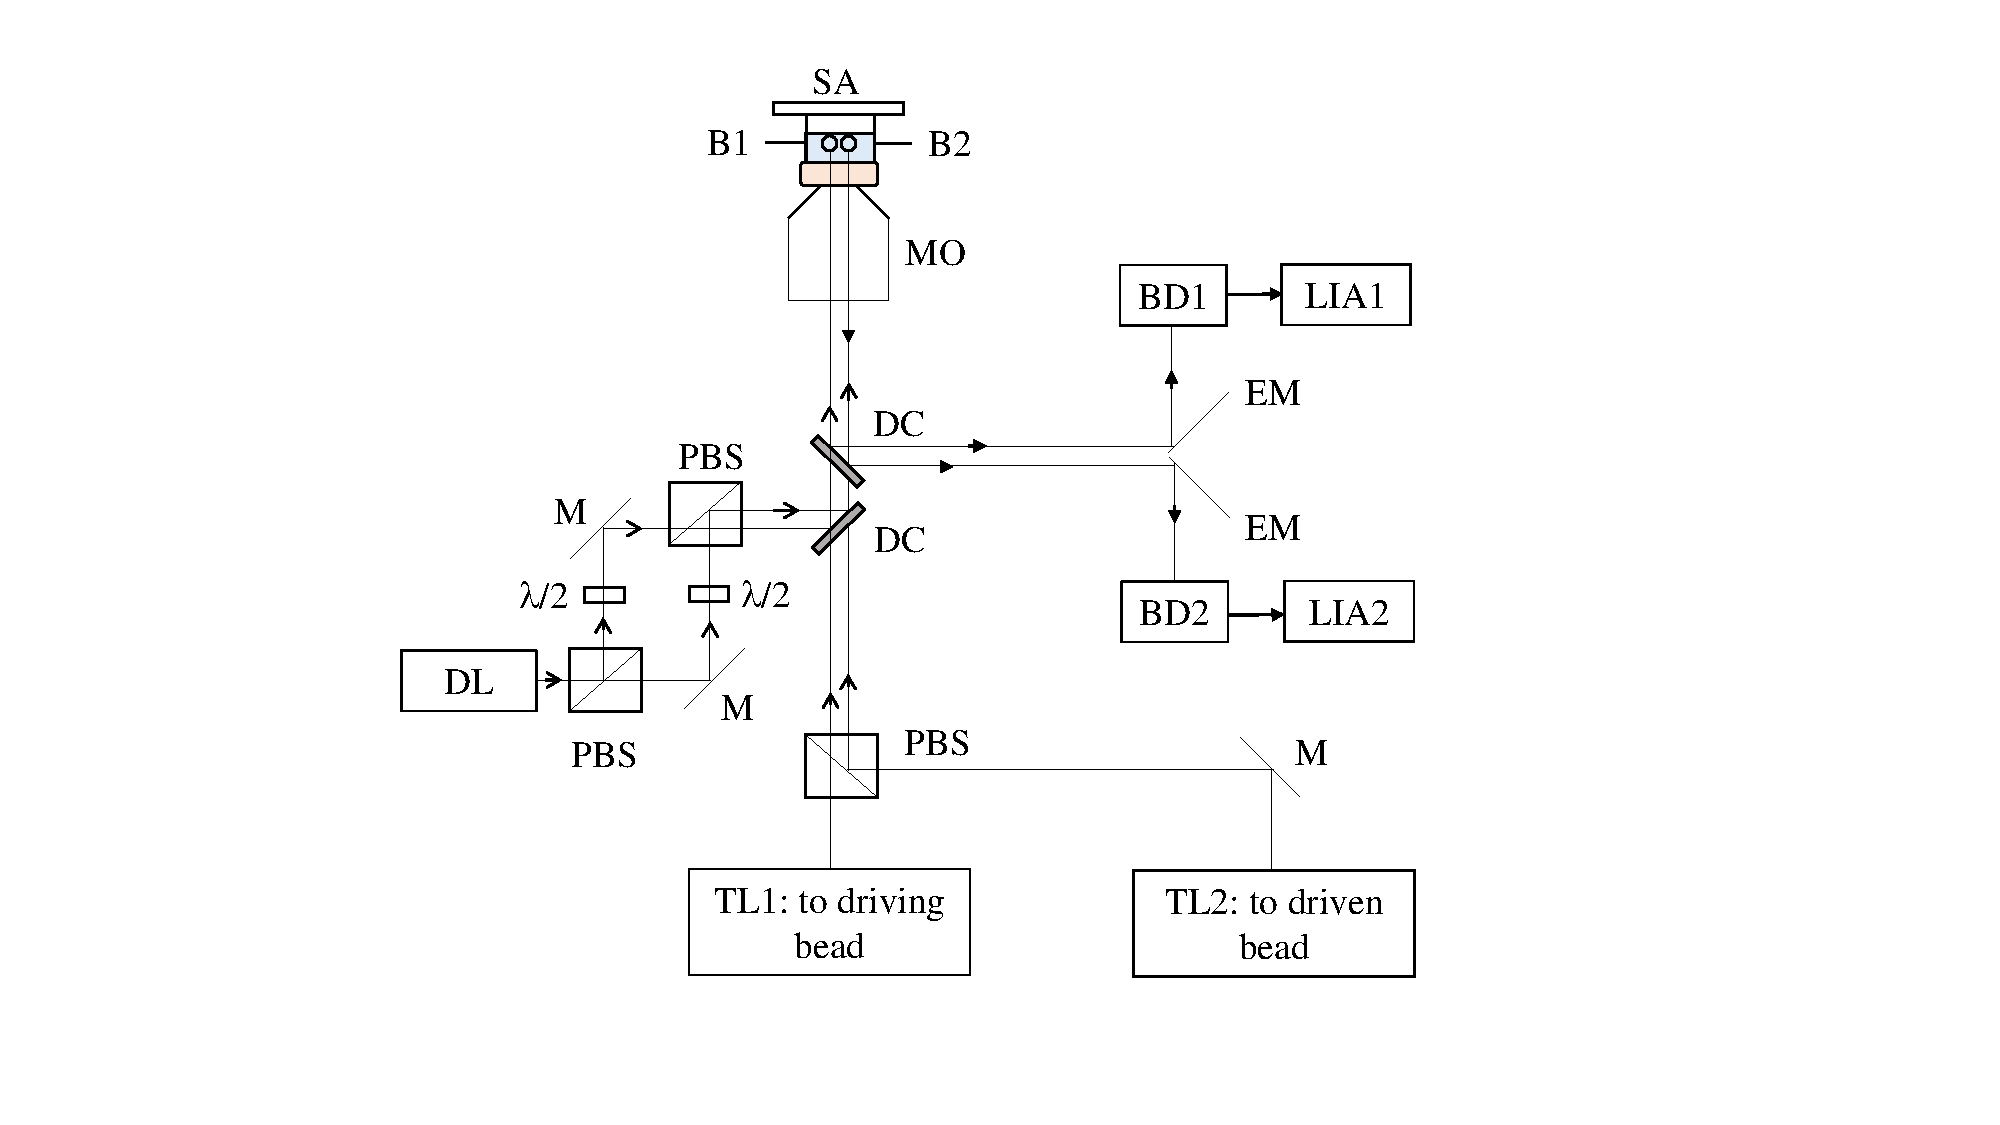
\includegraphics[width=0.35\textwidth]{fig1} \caption{A schematic diagram of the experimental setup. TL1: trapping laser
for driving particle B1, TL2: trapping laser for driven particle B2,
DL: detection laser, PBS: polarizing beam splitter cube, $\frac{\lambda}{2}$:
half wave plate, DC: dichroic mirror, MO: microscope objective, CS:
cover slip, BD1 and BD2: balanced detection systems based on Thorlabs
photodiodes PD-EC2, M: mirror, EM: edge mirror, LIA1 and LIA2: lock-in
amplifiers for B1 and B2, respectively.}
\label{Setup} 
\end{figure}

\textit{Experiment:} The details of the experimental setup towards
validation of the fluctuation response theorem are provided in Supplementary
Information - here we provide a brief description. Thus, we set up
a dual-beam optical tweezers (Fig. \ref{Setup}) by focusing two orthogonally
polarized beams of wavelength $\lambda=1064$ nm generated independently
from two diode lasers using a high NA immersion-oil microscope objective
(Zeiss PlanApo,$100\times1.4$). One of the lasers is modulated using
an AOM located conjugate to the back-focal plane of the microscope
objective, and a long optical path after the AOM ensures that a minimal
beam deflection is enough to modulate one of the trapped beams, so
that the intensity in the first order remains constant to around 2\%.
The modulated and unmodulated beams are independently coupled into
the trapping microscope using mirrors and a polarizing beam splitter,
while detection is performed using a separate laser at 671 nm generating
two detection beams also orthogonally polarized and superposed on
the respective trapping beams using dichroic beam splitters. The two
trapped beads are imaged and their displacements measured by back-focal-
plane-interferometry, with the imaging white light and detection beams
also separated at the output by dichroic beam splitters, which along
with the orthogonal polarization scheme ensures that cross-talk in
the detection beams is absent. A very low volume fraction sample ($\phi\approx0.01$)
is prepared with 3 $\mu$m diameter polystyrene latex beads in 1 M
NaCl-water solution for avoiding surface charges. We trap two spherical
polystyrene beads (Sigma LB-30) of mean size 3 $\mu$m each, in two
calibrated optical traps which are separated by a distance $4\pm0.1\:\mu$m,
so that the surface-surface distance of the trapped beads is $1\pm0.2\:\mu$m
($0.67a$, $a$ being the particle radius) and the distance from the
cover slip surface is 30 $\mu$m ($20a$, so as to overrule wall effects).
From the literature \cite{Stilgoe11}, the particle separation is
still large enough to avoid effects due to optical binding and surface
charges. In order to ensure that the trapping and detection beams
are not influencing each other, we measure the Brownian motion of
a trapped particle when the trapping and detection beams for the other
trap is switched on (in the absence of a particle), and check that
there are no changes in the measured trap stiffness. One of the traps
is sinusoidally modulated (amplitude around $0.2a$) and the phase
and amplitude response of both the driving and driven particles with
reference to the sinusoidal drive are measured by lock-in detection
(Stanford Research, SR830). To get large signal to noise, we use balanced
detection systems BD1 and BD2, for the driving and driven particles,
respectively. The voltage-amplitude calibration of our detection system
reveals that we can resolve motion of around 5 nm with an SNR of 2.
\begin{figure*}
\centering 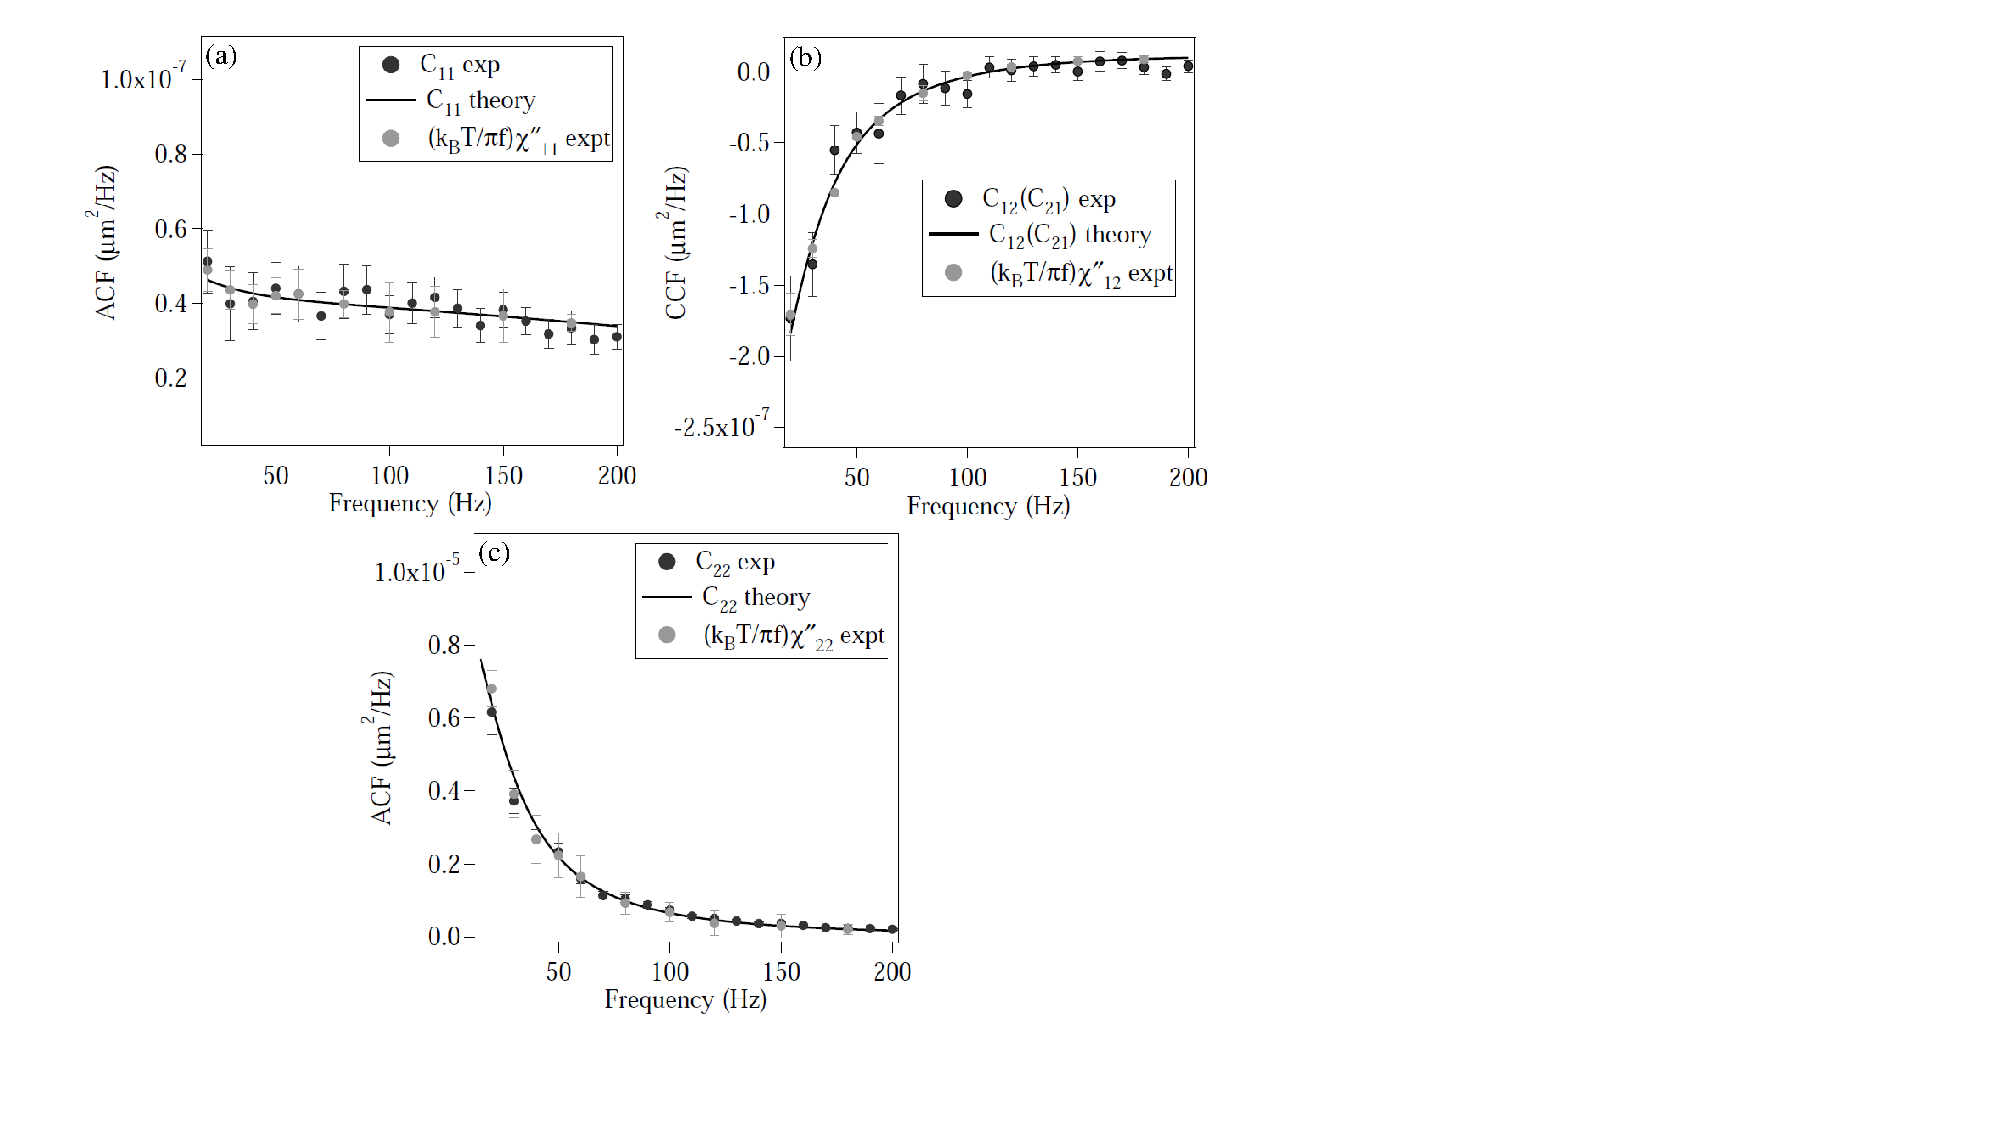
\includegraphics[scale=0.5]{fig2} \caption{Verification of the fluctuation-response relation $C_{ij}=(k_{B}T/\pi f)\chi_{ij}^{\prime\prime}$
for a pair of viscously coupled colloidal particles in optical traps.
The first and third panels compare the self-response and the position
auto-correlation of, respectively, the driving and driven colloid,
while the second panel compares their mutual-response and cross-correlation.
Theoretically computed correlation functions, assuming over-damped
motion of the colloids and slow viscous flow in the fluid, are shown
as solid lines. }
\label{fdt} 
\end{figure*}

Each of the optical traps are calibrated using equipartition and power
spectrum methods considering the the particle temperature to be same
as the room temperature. We verify that each of the potentials is
harmonic in nature from the histogram of the Brownian motion which
is satisfactorily Gaussian (Fig. 1 in Supplementary Information),
even when both trapping beams are on. The sampling frequency is 2
kHz, while we performed data blocking at the level of 100 points in
order to ensure good Lorentzian fits \cite{berg2004power} for trap
calibration. We maintain a considerably higher stiffness for the particle
in the modulated trap so that it is not affected by the back-flow
due to the driven particle. The low stiffness of the driven trap ensures
that it has a maximal response to the drive. Thus, for validation
of the fluctuation response theorem, the stiffness of the modulated
bead (B1) was 69.6 $\mu N/m$, while that of the driven is 4.8 $\mu N/m$.
Note that, to observe a clear amplitude resonance, a lower ratio of
trap stiffness is required, as we demonstrate later. The verification
of the fluctuation-response theorem is shown in Figs. \ref{fdt} .
It is understandable that while the fluctuation-response theorem is
in the form a simple equation for a single particle, for two particles
the equations would be represented in the form of a matrix, which
we discuss in more detail later. This is what we demonstrate in Fig.\ref{fdt}(a),
(b), and (c), where the auto and cross-correlations for both particles
are matched with the corresponding response functions. The auto-correlation
function of B1 is shown in Fig. \ref{fdt}(a), while that of B2 is
shown in Fig. \ref{fdt}(b). The corresponding response functions
($\mathit{\chi_{11}^{||},\:\chi{}_{22}^{||}}$) are obtained by measuring
the amplitude and phase of the individual particles when they are
themselves driven. Fig. \ref{fdt}(c) shows the cross-correlation
function which is again compared with the corresponding response function
$\mathit{\chi_{12}^{||}}$. This is obtained by measuring the amplitude
and phase of B2 when B1 is driven. Note that we are not able to measure
$\mathit{\chi_{21}^{||}}$which is the response of B1 when B2 is driven
since the much larger stiffness of B1 renders the amplitude of the
response extremely small so that it is beyond our detection sensitivity.
For the response measurements, each data point is the average of ten
separate measurements at each frequency. It is clear from the figures
that we obtain a good match between fluctuation and response - which
essentially validates the fluctuation-response relations for a pair
of colloidal particles coupled by hydrodynamic interactions. Note
that for consistency check, we also plot the cross-correlation function
in the time domain (Fig. 4 in Supplementary Information) and obtain
qualitatively similar data as reported in Ref. \cite{Meiners99}.

\textit{Theory:} The Langevin equations describing the stochastic
trajectories of the colloids are \cite{gardiner1985handbook}
\begin{align}
m_{i}\dot{\boldsymbol{v}_{i}} & +\boldsymbol{\gamma}_{ij}\cdot\boldsymbol{v}_{j}+{\bf \boldsymbol{\nabla}}_{i}U=\boldsymbol{{\bf \xi}}_{i}\label{eq1}
\end{align}
where $i,j=1,2$ refer to the driving and driven colloid, $m_{i}$
are their masses, $\boldsymbol{v}_{i}$ are their velocities, $\boldsymbol{\gamma}_{ij}$
are the second-rank friction tensors encoding the velocity-dependent
dissipative forces mediated by the fluid, $U=U_{1}+U_{2}$ is the
total potential of the conservative forces, and $\boldsymbol{\xi}_{i}$,
the Langevin noises, are zero-mean Gaussian random variables whose
variance is provided by the fluctuation-dissipation relation $\langle\boldsymbol{\xi}_{i}(t)\boldsymbol{\xi}_{j}(t^{\prime})\rangle=2k_{B}T\boldsymbol{\gamma}_{ij}\delta(t-t^{\prime})$.
The bold-face notation, with Cartesian indices suppressed, is used
for both vectors and tensors.

In the limit of slow viscous flow in the fluid, the friction tensors
can be calculated from the Stokes equation using a variety of methods
\cite{ladd1988,mazur1982,cichocki1994friction,singh2016crystallization,singh2016traction}.
To leading order the result is
\begin{equation}
\boldsymbol{\gamma}_{ij}=\delta_{ij}\boldsymbol{I}\gamma_{i}-(1-\delta_{ij})\gamma_{i}\gamma_{j}\mathcal{F}_{i}\mathcal{F}_{j}\boldsymbol{G}(\boldsymbol{r}_{i},\boldsymbol{r}_{j})
\end{equation}
where $\gamma_{i}=6\pi\eta a_{i}$ are the self-frictions, $\boldsymbol{G}$
is a Green's function of the Stokes equation \cite{pozrikidis1992},
$\boldsymbol{r}_{i}$ are the centers of the colloids and $\mathcal{F}_{i}=1+\frac{a_{i}^{2}}{6}\nabla_{i}^{2}$
are the Fax�n corrections that account for the finite radius, $a_{i}$,
of the colloids. We emphasize that this expression is not limited
to the translationally invariant Green's function of unbounded flow,
$8\pi\eta\,\boldsymbol{G}(\boldsymbol{r})=(\nabla^{2}\boldsymbol{I}-\boldsymbol{\nabla\nabla})r$,
but holds generally for any Green's function and is both symmetric
and positive-definite \cite{singh2016crystallization,singh2016traction}.
The mutual friction tensors decay inversely with distance in an unbounded
fluid and more rapidly in the proximity of boundaries. The assumption
of slow viscous flow is valid at frequencies $\omega\tau_{\nu}\ll1$
where $\tau_{\nu}=\rho L^{2}/\eta$ is the vorticity diffusion time
scale \cite{kim2005}. 

The harmonic optical potentials are given by $U_{i}(t)=\frac{1}{2}k_{i}|{\bf \boldsymbol{r}}_{i}-{\bf \boldsymbol{r}}_{i}^{0}|^{2}$
where $\boldsymbol{r}_{i}^{0}$ are the centers and $k_{i}$ are the
stiffnesses of the optical traps. Note the absence of conservative
mutual couplings. The system remains in equilibrium when the trap
centers are stationary but is driven into non-equilibrium when they
are modulated in time as $\boldsymbol{r}_{i}^{0}(t)$. For small modulations
the response is linear. 

For modulation frequencies $\omega\ll\gamma_{i}/m_{i}$ the velocities
can be adiabatically eliminated from the inertial Langevin equations
to yield inertialess Langevin equations for the positions \cite{gardiner1984adiabatic}.
The multiplicative noises in the resulting equations have clear interpretations
within the adiabatic elimination procedure; there is no It�-Stratonovich
dilemma \cite{van1981ito,gardiner1985handbook,van1992stochastic,klimontovich1990ito,klimontovich1994nonlinear}.
Both correlation and response functions can be calculated in this
limit. Linearizing about the mean separation between the trap centers
and decomposing the motion into components parallel and perpendicular
to the separation vector, the result for the parallel response function
is

\begin{gather}
\text{Im}\left[\chi_{ij}^{||}(\omega)\right]=\frac{\omega M_{ij}}{(\text{det}A-\omega^{2})^{2}+(\omega\begin{tabular}{c}
 tr\end{tabular}A)^{2}}\\
\nonumber 
\end{gather}
where $A_{ij}=\mu_{ij}^{||}k_{j}$ is a ``response'' matrix, the
mobility matrix $\mu_{ij}^{||}$ is the inverse of the friction matrix
and
\[
M_{ij}=\left(\begin{array}{cc}
\begin{tabular}{c}
 \ensuremath{\tfrac{k_{2}}{k_{1}}\mu_{22}^{\parallel}}\end{tabular}\text{det}A+\mu_{11}^{\parallel}\omega^{2} & -\mu_{12}^{\parallel}(\text{det}A-\omega^{2})\\
\, & \,\\
-\mu_{21}^{\parallel}(\text{det}A-\omega^{2}) & \begin{tabular}{c}
 \ensuremath{\tfrac{k_{1}}{k_{2}}\mu_{11}^{\parallel}}\end{tabular}\text{det}A+\mu_{22}^{\parallel}\omega^{2}
\end{array}\right).
\]
The magnitude of the response of the driven bead to the driving bead
is maximum at the ``resonance'' frequency

\begin{equation}
\omega_{res}=\sqrt{\text{det}A}=\sqrt{\mu_{11}^{\parallel}\mu_{22}^{\parallel}k_{1}k_{2}\left(1-\frac{\mu_{12}^{\parallel}\mu_{21}^{\parallel}}{\mu_{11}^{\parallel}\mu_{22}^{\parallel}}\right)}.
\end{equation}
A simple analysis of the system with the two particles executing Brownian
motion in the absence of the external drive leads us to write down
the auto and cross-correlation functions ($C_{ij}$), so that by comparing
with the response functions $\chi_{ij}^{\prime\prime}$, we have $C_{ij}=(k_{B}T/\pi f)\chi_{ij}^{\prime\prime}$
which is the well known fluctuation-response relationship \cite{chaikin2000principles}.

\begin{figure}
\centering 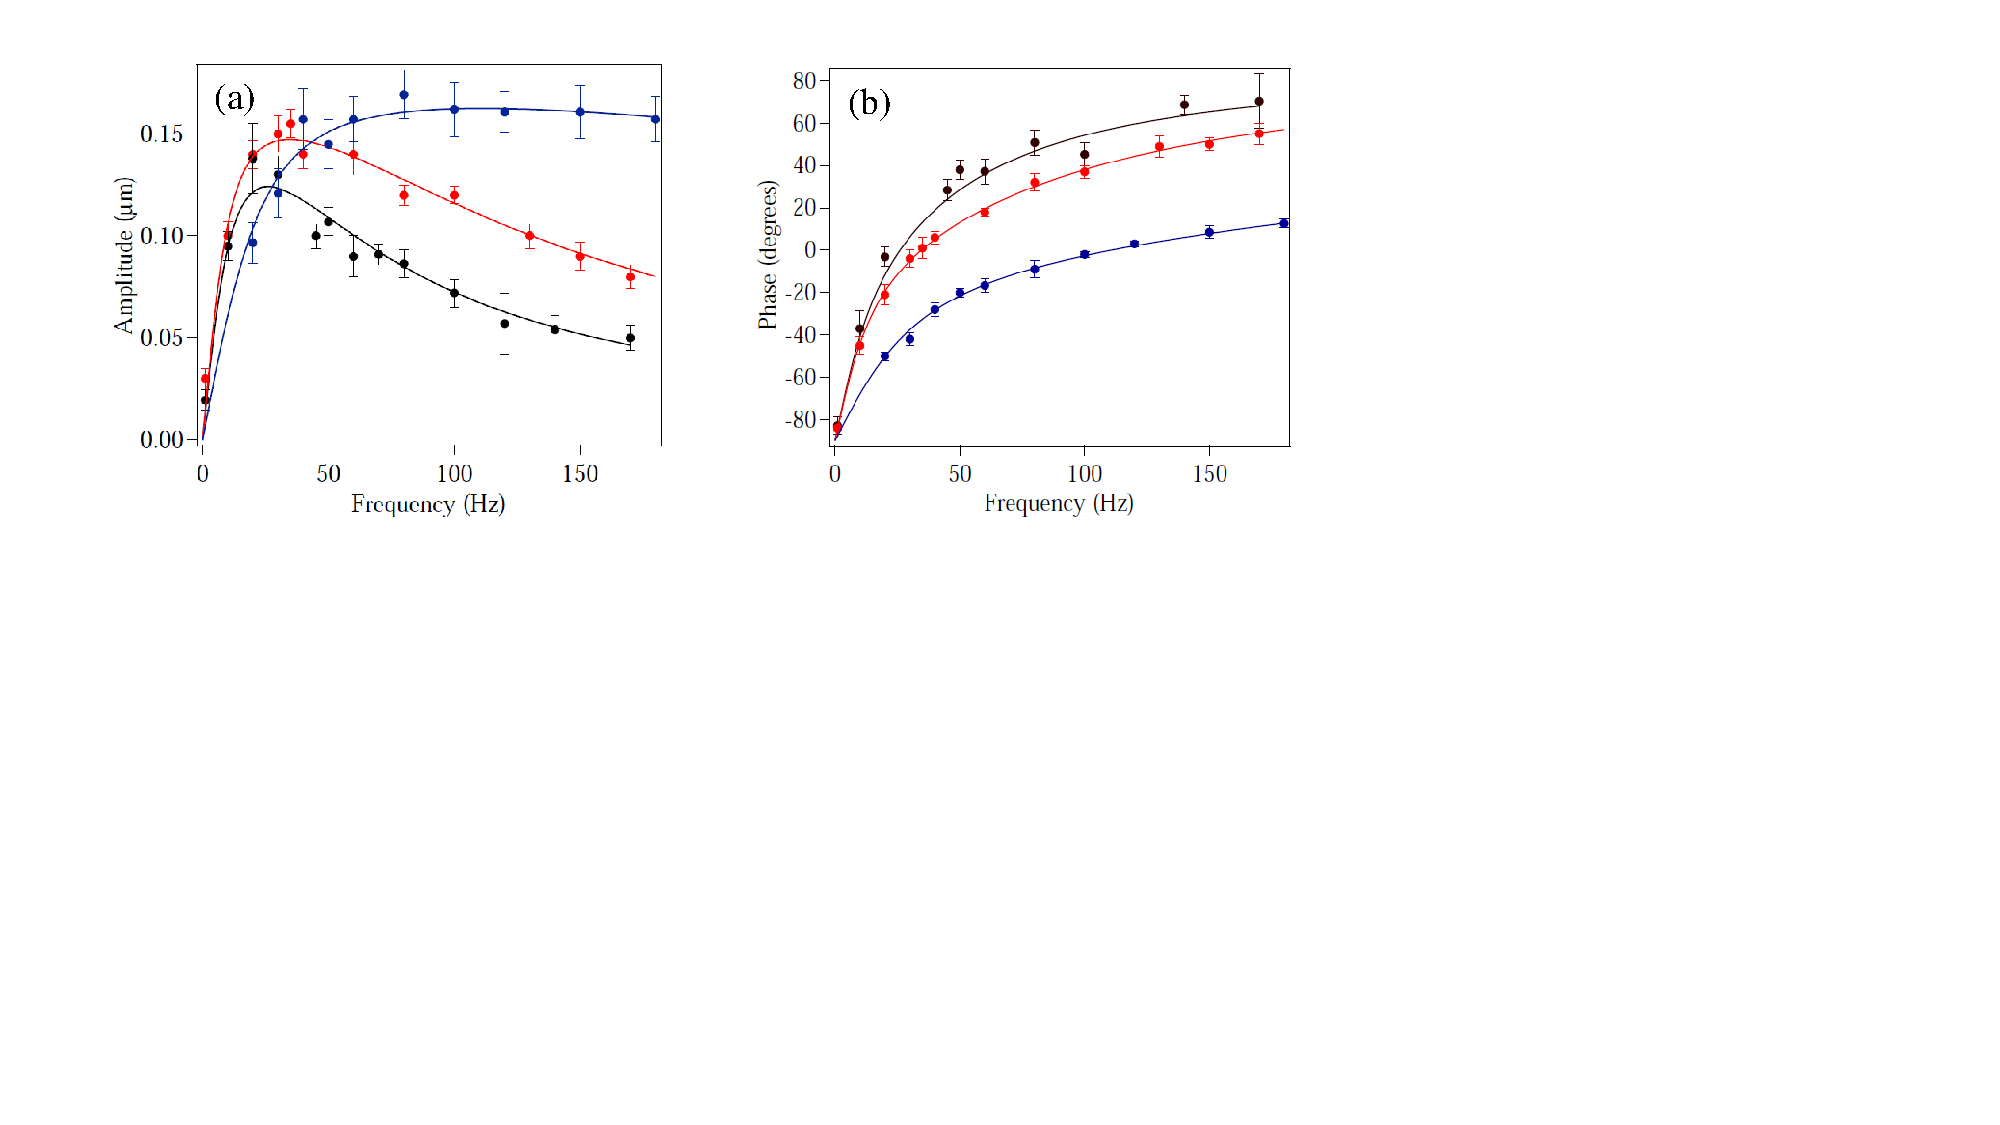
\includegraphics[width=0.45\textwidth]{fig3} \caption{Amplitude and phase response for driven (B2) bead for different trap
stiffness ratios with the inter-particle separation $0.67a$. (a)
and (b) demonstrate amplitude and phase responses (with respect to
driving frequency) of B2, for trap stiffness ratios of 2.5:1 (black),
5.7:1 (red), and 14.5:1 (blue) for (c) and (e). The resonance frequency
in (c) is 20 Hz (black), 35 Hz (red), and 111 Hz (blue). The solid
spheres denote experimental data points while the solid lines are
corresponding theoretical fits. }
\label{response}
\end{figure}
This is indeed what we validate in Fig.\ref{response}(a)-(c). We
now focus on a particularly interesting facet of our problem, namely
the amplitude and phase response of B2 under the influence of the
driven particle B1. We study this experimentally for three different
trap stiffness ratios of B1 and B2, the results of which are shown
in Fig. \ref{response}(a) and (b). Note that we fit each graph with
the calculated values of the responses for the experimental parameters
used, and obtain very good fits. The amplitude and phase response
of B1 (Supplementary information) to the drive frequency is expected,
with the amplitude decaying with increasing frequency, and the phase
being in sync with the drive at low frequencies and gradually lagging
behind as the frequency is increased. However, the amplitude response
of B2 is rather interesting, and shows a clear resonance response
at a certain frequency, the value of which increases as the stiffness
ratio of the traps is increased. Thus, we have a resonance frequency
of around 111 Hz (blue solid spheres in Fig.\ref{response}(c)) with
$\mathit{k_{1}:k_{2}}=$14.5, a frequency of around 33 Hz with a ratio
of 5.7:1 (red solid spheres), and a frequency of around 20 Hz with
a ratio of 2.5:1 (black solid spheres). In fact, it is as if the entrained
fluid has minimum impedance around this frequency, so that there is
maximum energy transfer between the driving and the driven beads.
The amplitude of the resonance is also linearly dependent on the particle
separation, and falls off as the latter is increased, so that in our
current detection sensitivity, we do not observe the resonance effects
beyond a surface-surface separation greater than $3a$ - this increased
distance also being smaller than that used in earlier experiments,
which possibly explains the fact that this phenomenon has not been
reported earlier. The width of the resonance ($\mathit{Q}$ factor)
is dependent on the stiffness ratio, and increases as the latter is
reduced. For a given medium, the resonance can thus be tuned by changing
the stiffness ratios. Interestingly, it is obvious that the value
of the $\mathit{Q}$-factor as well as the resonance frequency also
depends on the damping, and can be modified by changing the viscosity
of the solution. This property promises the measurement of this frequency
shift as an accurate two-point micro-rheology probe of local viscosity
of a fluid. Finally, the phase response in \ref{response}(e) is easily
explained: B2 lags 90 degrees in phase with respect to the drive at
very low frequencies with the lag reducing until the drive and driven
are in phase at resonance, after which the driven bead leads in phase,
and asymptotically approaches 90 degrees at high frequencies. The
rate of approach is also determined by the stiffness ratio, and is
rather slow at large stiffness ratios. Indeed, this is exactly similar
to the relationship between velocity and driving force for a forced
damped harmonic oscillator, and arises due to the fact that the oscillators
are dissipatively coupled. 

In conclusion, we perform a direct experimental verification of the
fluctuation-dissipation relation in a system consisting of two colloidal
particles confined in a viscous medium (water) in very close proximity
(surface-surface separation less than the particle radius) using separate
optical tweezers. Our results provide a confirmation of the validity
of the fluctuation-dissipation relation in the presence of long-ranged
dissipative forces that are the only source of coupling of, otherwise,
independent degrees of freedom. Surprisingly, we identify a resonance
in the response in system which is overdamped and suggest its use
in accurate two-point microrheology. The present experiment can be
extended in several directions: holographic traps can be used to test
the fluctuation-dissipation relation in the presence of many-body
hydrodynamic interactions, measurements at higher frequencies can
uncover the effects of retarded hydrodynamic interactions and the
role of particle inertia. Some of these will be presented in forthcoming
work. 

This work was supported by the Indian Institute of Science Education
and Research, Kolkata, an autonomous research and teaching institute
funded by the Ministry of Human Resource Development, Govt. of India.

\bibliographystyle{apsrev4-1}
\bibliography{2bead-fdt}

\end{document}
